\documentclass[aspectratio=169,10pt]{beamer}

\usepackage{fontspec}
\usepackage[french]{babel}
\usepackage{array}
\usepackage{booktabs}
\usepackage{listings}
\usepackage{appendixnumberbeamer}
\usepackage{tikz}
\usetikzlibrary{arrows.meta,positioning,fit}

\definecolor{accent}{HTML}{1F4E79}
\definecolor{accent2}{HTML}{C8553D}
\definecolor{soft}{HTML}{EAF0F6}
\definecolor{codebg}{HTML}{F5F7FA}

% Speaker of the current part, shown in the footline.
\newcommand{\speaker}{}

\setbeamertemplate{navigation symbols}{}
\setbeamercolor{structure}{fg=accent}
\setbeamercolor{frametitle}{fg=accent}
\setbeamerfont{frametitle}{series=\bfseries,size=\Large}
\setbeamercolor{title}{fg=accent}
\setbeamerfont{title}{series=\bfseries,size=\LARGE}
\setbeamertemplate{itemize item}{\color{accent2}\small$\blacktriangleright$}
\setbeamertemplate{itemize subitem}{\color{accent}\textendash}
\setbeamertemplate{footline}{%
  \hspace*{1em}\color{gray}\scriptsize Compression DCT + CSR en C++\hfill
  {\color{accent2}\bfseries\speaker}\hfill
  \insertframenumber\,/\,\inserttotalframenumber\hspace*{1em}\vspace*{0.7em}}

\lstset{
  language=C++,
  basicstyle=\ttfamily\scriptsize,
  backgroundcolor=\color{codebg},
  keywordstyle=\color{accent}\bfseries,
  commentstyle=\color{gray}\itshape,
  stringstyle=\color{accent2},
  morekeywords={noexcept,override,explicit,constexpr,nullptr,delete,default},
  columns=fullflexible,
  keepspaces=true,
  xleftmargin=0.4em,
  framexleftmargin=0.4em,
  aboveskip=0.3em,
  belowskip=0.3em,
}

\tikzset{
  box/.style={draw=accent, fill=soft, rounded corners=2pt, align=center, font=\scriptsize, inner sep=4pt},
  stage/.style={box, minimum width=2.1cm, minimum height=1.05cm},
  abstract/.style={box, fill=white, dashed},
  flow/.style={-{Stealth[length=2mm]}, accent, thick},
  link/.style={-{Stealth[length=1.6mm]}, gray},
}

\newcommand{\code}[1]{\texttt{#1}}

\title{Compression d'image par DCT et stockage CSR en C++}
\subtitle{Conception du code et représentation des données}
\author{Romain Ben \and Karim Zrig}
\institute{MAM4 Polytech Nice Sophia \quad|\quad Projet C++}
\date{23 septembre 2026}

\begin{document}

\renewcommand{\speaker}{Romain}

\begin{frame}
  \titlepage
\end{frame}

\begin{frame}{Du projet Python au C++}
  \begin{columns}[T]
    \begin{column}{0.46\textwidth}
      \textbf{MAM3 : version Python}
      \begin{itemize}
        \item DCT, quantification, troncature avec \code{numpy}
        \item stockage creux avec \code{scipy.sparse}
        \item application Streamlit
      \end{itemize}
    \end{column}
    \begin{column}{0.48\textwidth}
      \textbf{MAM4 : version C++20}
      \begin{itemize}
        \item même algorithme, aucune bibliothèque de calcul
        \item but : apprendre le C++ sur un problème connu
        \item programme en ligne de commande \code{jpeg\_csr}
      \end{itemize}
    \end{column}
  \end{columns}

  \vspace{1.4em}
  \centering
  \begin{tikzpicture}[node distance=0.6cm]
    \node[box, minimum width=5.6cm, minimum height=1.2cm, font=\small] (p1)
      {\textbf{1. Romain}\\ organisation du code\\ représentation des données};
    \node[box, minimum width=5.6cm, minimum height=1.2cm, font=\small, right=of p1] (p2)
      {\textbf{2. Karim}\\ matrice creuse, ressources,\\ polymorphisme, résultats};
  \end{tikzpicture}
\end{frame}

\begin{frame}{L'algorithme en une slide}
  \centering
  \begin{tikzpicture}[node distance=0.45cm]
    \node[stage] (img) {Image RGB\\[1pt] blocs $8\times8$\\ centrage $-128$};
    \node[stage, right=of img] (dct) {DCT\\[1pt] $D = P M P^{T}$};
    \node[stage, right=of dct] (q) {Quantification\\[1pt] $\operatorname{trunc}(D / \alpha Q)$};
    \node[stage, right=of q] (mask) {Seuil $S$\\ masque $F$};
    \node[stage, right=of mask, fill=accent, text=white] (csr) {CSR\\ 3 canaux\\ fichier \code{.csr}};
    \draw[flow] (img) -- (dct);
    \draw[flow] (dct) -- (q);
    \draw[flow] (q) -- (mask);
    \draw[flow] (mask) -- (csr);

    \node[stage, below=1.1cm of csr] (read) {Relecture\\ du \code{.csr}};
    \node[stage, left=of read] (mult) {$\hat D \odot \alpha Q$};
    \node[stage, left=of mult] (idct) {DCT inverse\\[1pt] $M = P^{T} D P$};
    \node[stage, left=of idct] (clip) {$+128$\\ bornage $[0, 255]$};
    \node[stage, left=of clip] (png) {Image\\ reconstruite};
    \draw[flow] (csr) -- (read);
    \draw[flow] (read) -- (mult);
    \draw[flow] (mult) -- (idct);
    \draw[flow] (idct) -- (clip);
    \draw[flow] (clip) -- (png);
  \end{tikzpicture}

  \vspace{0.8em}
  \small
  $P$ est orthogonale : l'inverse de la DCT est sa transposée.\\[0.3em]
  Masque carré (Python) : $k, l < F$ \qquad Masque triangulaire (sujet) : $k + l < F$
\end{frame}

\begin{frame}{Organisation du code}
  \centering
  \begin{tikzpicture}[node distance=0.5cm and 0.7cm]
    \node[box, minimum width=2.6cm] (io) {\code{image\_io}\\ \code{load\_image}, \code{save\_png}\\ {\tiny seul fichier qui voit stb}};
    \node[box, minimum width=2.6cm, below=of io] (image) {\code{Image}\\ {\tiny RGB, \code{std::vector<double>}}};
    \node[box, minimum width=2.6cm, below=of image] (table) {\code{QuantizationTable}\\ {\tiny diviseurs $\geq 1$, facteur $\alpha$}};

    \node[box, minimum width=3cm, minimum height=1.4cm, right=1.4cm of image, fill=accent, text=white] (codec)
      {\code{codec}\\[2pt] \code{compress}\\ \code{decompress}};
    \node[box, above=of codec] (dct) {\code{Dct} \quad \code{Matrix8}\\ {\tiny \code{std::array}, $P$ calculée une fois}};
    \node[abstract, below=0.9cm of codec] (mask) {\code{FrequencyMask}\\ {\tiny interface abstraite}};
    \node[box, below left=0.55cm and -0.4cm of mask] (square) {\code{SquareMask}};
    \node[box, below right=0.55cm and -0.4cm of mask] (triangle) {\code{TriangleMask}};

    \node[box, minimum width=3.2cm, right=1.4cm of codec] (compressed)
      {\code{CompressedImage}\\ {\tiny 3 $\times$ \code{SparseMatrix} (CSR) + $Q$}};
    \node[box, above=of compressed] (file) {fichier \code{.csr}\\ {\tiny \code{save\_compressed}, \code{load\_compressed}}};
    \node[box, below=of compressed] (metrics) {\code{metrics} \quad \code{noise}\\ {\tiny erreur $L^2$, PSNR, poivre et sel}};

    \node[box, right=0.9cm of compressed, minimum height=2.2cm] (main) {\code{main}\\ \code{options}\\[2pt] {\tiny ligne de}\\ {\tiny commande}};

    \draw[link] (io) -- (image);
    \draw[flow] (image) -- (codec);
    \draw[flow] (table) -| ([xshift=-0.6cm]codec.south);
    \draw[link] (dct) -- (codec);
    \draw[flow] (mask) -- node[right, font=\tiny, text=gray] {\code{const\&}} (codec);
    \draw[link] (square) -- (mask);
    \draw[link] (triangle) -- (mask);
    \draw[flow, <->] (codec) -- (compressed);
    \draw[link, <->] (compressed) -- (file);
    \draw[link] (main) -- (compressed);
  \end{tikzpicture}

  \vspace{0.5em}
  \small
  Compilation séparée : \code{include/} (en-têtes commentés) et \code{src/} \quad|\quad
  espace de noms \code{jpeg} \quad|\quad \code{Makefile} : \code{jpeg\_csr} et \code{run\_tests}
  à partir des mêmes objets
\end{frame}

\begin{frame}[fragile]{Représenter l'image : un seul \code{std::vector}}
  \begin{columns}[T]
    \begin{column}{0.5\textwidth}
\begin{lstlisting}
class Image {
public:
    double& operator()(std::size_t row,
        std::size_t col, std::size_t channel);
    const double& operator()(std::size_t row,
        std::size_t col, std::size_t channel) const;
    // + at(): checked access

private:
    std::size_t width_;
    std::size_t height_;
    std::vector<double> pixels_;
    // invariant: size == width * height * 3
};
\end{lstlisting}
    \end{column}
    \begin{column}{0.46\textwidth}
      \begin{itemize}
        \item pas de vecteur de vecteurs : une seule allocation, lignes toujours de même taille
        \item mémoire contiguë, un seul invariant
        \item deux surcharges de \code{operator()} : écrire, ou lire une image \code{const}
        \item \code{at()} vérifie les bornes, comme \code{std::vector}
      \end{itemize}
    \end{column}
  \end{columns}

  \vspace{0.6em}
  \centering
  \begin{tikzpicture}[x=0.5cm, y=0.5cm,
      cell/.style={draw=accent, minimum width=0.5cm, minimum height=0.5cm, font=\tiny\ttfamily, inner sep=0pt, anchor=south west}]
    \foreach \x/\ch/\col in {0/R/red!20, 1/G/green!20, 2/B/blue!15, 3/R/red!20, 4/G/green!20, 5/B/blue!15} {
      \node[cell, fill=\col] at (\x, 0) {\ch};
    }
    \node[font=\scriptsize] at (7, 0.5) {\dots};
    \foreach \x/\ch/\col in {8/R/red!20, 9/G/green!20, 10/B/blue!15} {
      \node[cell, fill=\col] at (\x, 0) {\ch};
    }
    \node[font=\scriptsize] at (12, 0.5) {\dots};
    \node[font=\tiny, anchor=north] at (1.5, 0) {pixel (0, 0)};
    \node[font=\tiny, anchor=north] at (4.5, 0) {pixel (0, 1)};
    \node[font=\tiny, anchor=north] at (9.5, 0) {pixel (1, 0)};
    \node[font=\small, anchor=west] at (13.5, 0.5) {indice $= (\mathit{row} \times w + \mathit{col}) \times 3 + \mathit{channel}$};
  \end{tikzpicture}
\end{frame}

\begin{frame}[fragile]{Le bloc \texorpdfstring{$8\times8$}{8x8} : \code{std::array}, aucune allocation}
  \begin{columns}[T]
    \begin{column}{0.5\textwidth}
\begin{lstlisting}
class Matrix8 {
    ...
private:
    std::array<double, 64> values_{};
};
Matrix8 operator*(const Matrix8& lhs,
                  const Matrix8& rhs);

class Dct {
public:
    Dct();   // computes P and P^T once
    Matrix8 forward(const Matrix8& block) const;
    Matrix8 inverse(
        const Matrix8& coefficients) const;
private:
    // declaration order = initialization order
    Matrix8 p_;
    Matrix8 p_transposed_;
};
\end{lstlisting}
    \end{column}
    \begin{column}{0.46\textwidth}
      \begin{itemize}
        \item un seul type pour un bloc de pixels, $P$ et les coefficients
        \item taille connue à la compilation : pas d'allocation, alors qu'une image $512\times512$
          compte 12\,288 blocs
        \item \code{operator*} libre : \code{p\_ * block * p\_transposed\_} s'écrit comme la formule
        \item piège appris : les membres sont initialisés dans l'ordre de leur \textbf{déclaration}
      \end{itemize}
    \end{column}
  \end{columns}
\end{frame}

\begin{frame}[fragile]{Quantification : un invariant qui fixe un type}
  \begin{columns}[T]
    \begin{column}{0.5\textwidth}
\begin{lstlisting}
// Invariant: all divisors are >= 1.
class QuantizationTable {
public:
    // throws std::invalid_argument otherwise
    explicit QuantizationTable(
        const Matrix8& divisors);

    static QuantizationTable standard();
    static QuantizationTable uniform(double value);

    // new table alpha * Q, invariant checked again
    QuantizationTable scaled(double alpha) const;

private:
    Matrix8 divisors_;
};
\end{lstlisting}
    \end{column}
    \begin{column}{0.46\textwidth}
      \centering
      \begin{tikzpicture}[node distance=0.35cm]
        \node[box, minimum width=4.6cm] (a) {diviseurs $Q_{k,l} \geq 1$};
        \node[box, minimum width=4.6cm, below=of a] (b) {$|D_{k,l}| \leq 8 \times 128 = 1024$};
        \node[box, minimum width=4.6cm, below=of b, fill=accent, text=white] (c) {$|D_{k,l} / Q_{k,l}| \leq 1024$ : tient dans \code{std::int16\_t}};
        \draw[flow] (a) -- (b);
        \draw[flow] (b) -- (c);
      \end{tikzpicture}

      \vspace{0.6em}
      \raggedright
      \begin{itemize}
        \item vérifié une fois, dans le constructeur
        \item \code{explicit} : pas de conversion implicite
        \item fonctions statiques : une par matrice du projet MAM3
      \end{itemize}
    \end{column}
  \end{columns}
\end{frame}

\renewcommand{\speaker}{Karim}

\begin{frame}[fragile]{La matrice creuse CSR, écrite à la main}
  \begin{columns}[T]
    \begin{column}{0.52\textwidth}
\begin{lstlisting}
class SparseMatrix {
public:
    // dense matrix: only read
    SparseMatrix(std::size_t rows, std::size_t cols,
        const std::vector<std::int16_t>& dense);

    // arrays read in a file: taken by value,
    // then moved (std::move), checked
    SparseMatrix(std::size_t rows, std::size_t cols,
        std::vector<std::int16_t> values,
        std::vector<std::int32_t> column_indices,
        std::vector<std::int32_t> row_pointers);
private:
    std::vector<std::int16_t> values_;
    std::vector<std::int32_t> column_indices_;
    std::vector<std::int32_t> row_pointers_;
};
\end{lstlisting}
    \end{column}
    \begin{column}{0.45\textwidth}
      {\centering\scriptsize
        $\begin{pmatrix} 5 & 0 & 0\\ 0 & 0 & 0\\ 0 & 3 & 7 \end{pmatrix}$%
        \enspace$\rightarrow$\enspace
        {%
        \begin{tabular}{@{}r@{\;=\;}l@{}}
          \code{values} & $\{5, 3, 7\}$\\
          \code{column\_indices} & $\{0, 1, 2\}$\\
          \code{row\_pointers} & $\{0, 1, 1, 3\}$
        \end{tabular}}\par}
      \vspace{0.6em}
      \small
      \begin{itemize}
        \item remplace \code{scipy.sparse.csr\_matrix}, mêmes types
        \item environ 95\,\% de zéros : seuls les autres sont stockés
        \item invariant : pointeurs croissants, colonnes triées, aucun zéro stocké
        \item déplacement : aucun élément recopié à la relecture
      \end{itemize}
    \end{column}
  \end{columns}
\end{frame}

\begin{frame}{Image compressée et fichier \code{.csr}}
  \begin{columns}[T]
    \begin{column}{0.46\textwidth}
      \textbf{Composition}
      \begin{itemize}
        \item \code{CompressedImage} = dimensions + $Q$ + \code{std::vector} de 3 \code{SparseMatrix}
        \item invariant : multiples de 8, trois canaux de la taille de l'image
      \end{itemize}
      \vspace{0.6em}
      \textbf{Flux binaires}
      \begin{itemize}
        \item \code{write} et \code{read} surchargées : le compilateur choisit selon le type
        \item \code{std::ofstream} ferme le fichier tout seul (RAII)
      \end{itemize}
    \end{column}
    \begin{column}{0.5\textwidth}
      \small
      \begin{tabular}{@{}ll@{}}
        \toprule
        Contenu du fichier & Type \\
        \midrule
        signature \code{JCSR} & 4 octets \\
        largeur, hauteur & \code{uint32} \\
        matrice $Q$ & 64 \code{double} \\
        \multicolumn{2}{@{}l}{pour chaque canal R, G, B :} \\
        \quad \code{nnz} & \code{uint32} \\
        \quad pointeurs de lignes & \code{int32} \\
        \quad colonnes & \code{int32} \\
        \quad valeurs & \code{int16} \\
        \bottomrule
      \end{tabular}

      \vspace{0.8em}
      Relecture : dimensions bornées \textbf{avant} toute allocation, puis chaque constructeur
      revérifie son invariant. Un fichier corrompu lance une exception.
    \end{column}
  \end{columns}
\end{frame}

\begin{frame}[fragile]{Ressources : RAII et règle de zéro}
  \begin{columns}[T]
    \begin{column}{0.52\textwidth}
\begin{lstlisting}
// Array allocated by stbi_load: freed by the
// destructor, even if an exception is thrown.
class StbPixels {
public:
    explicit StbPixels(const std::string& path);
    ~StbPixels();   // stbi_image_free(data_)

    StbPixels(const StbPixels&) = delete;
    StbPixels& operator=(const StbPixels&) = delete;

private:
    int width_{};
    int height_{};
    unsigned char* data_{nullptr};
};
\end{lstlisting}
    \end{column}
    \begin{column}{0.44\textwidth}
      \textbf{Règle de zéro partout ailleurs}
      \begin{itemize}
        \item \code{std::vector} et \code{std::array} gèrent la mémoire
        \item aucun destructeur ni copie écrits
        \item aucun \code{new} ni \code{delete} dans le programme
      \end{itemize}
      \vspace{0.6em}
      \textbf{Une seule ressource brute}
      \begin{itemize}
        \item le tableau de pixels de stb, confié à \code{StbPixels}
        \item copie interdite : deux objets libéreraient le même tableau (TD 4)
      \end{itemize}
    \end{column}
  \end{columns}
\end{frame}

\begin{frame}[fragile]{Polymorphisme : le masque est choisi à l'exécution}
  \begin{columns}[T]
    \begin{column}{0.46\textwidth}
\begin{lstlisting}
class FrequencyMask {
public:
    virtual bool keeps(std::size_t k,
                       std::size_t l) const = 0;
    virtual std::string name() const = 0;
    virtual ~FrequencyMask() = default;
};

class SquareMask : public FrequencyMask { ... };
class TriangleMask : public FrequencyMask { ... };

CompressedImage compress(const Image& image,
    const QuantizationTable& table,
    int threshold, const FrequencyMask& mask);
\end{lstlisting}
    \end{column}
    \begin{column}{0.5\textwidth}
\begin{lstlisting}
// main.cpp
if (options.mask == MaskKind::triangle) {
    const TriangleMask mask{options.cutoff};
    return compress_with_mask(options, mask);
}
const SquareMask mask{options.cutoff};
return compress_with_mask(options, mask);
\end{lstlisting}
      \begin{itemize}
        \item même démarche que \code{ScalarFunction} au TD 6
        \item \code{compress} ne nomme aucun masque : en ajouter un ne la modifie pas
        \item objet local passé par référence : pas de \code{new}, pas de copie, pas de slicing
      \end{itemize}
    \end{column}
  \end{columns}
\end{frame}

\begin{frame}{Validation et résultats}
  \begin{columns}[T]
    \begin{column}{0.31\textwidth}
      \centering
      {\Huge\bfseries\color{accent} 17}\\[0.2em]
      \small fonctions de test\\[0.3em]
      \scriptsize tests Python repris, invariants, fichier \code{.csr} ; CI sous AddressSanitizer
      et UBSan, 91\,\% de couverture
    \end{column}
    \begin{column}{0.33\textwidth}
      \centering
      {\Huge\bfseries\color{accent} 25}\\[0.2em]
      \small coefficients différents sur 786\,432\\[0.3em]
      \scriptsize écart de 1, dû à un arrondi flottant côté Python ($/255$ puis $\times 255$)
    \end{column}
    \begin{column}{0.31\textwidth}
      \centering
      {\Huge\bfseries\color{accent} $\times$11}\\[0.2em]
      \small plus rapide que Python\\[0.3em]
      \scriptsize 50\,ms contre 543\,ms pour compresser et décompresser une image $512\times512$
    \end{column}
  \end{columns}

  \vspace{0.9em}
  \centering
  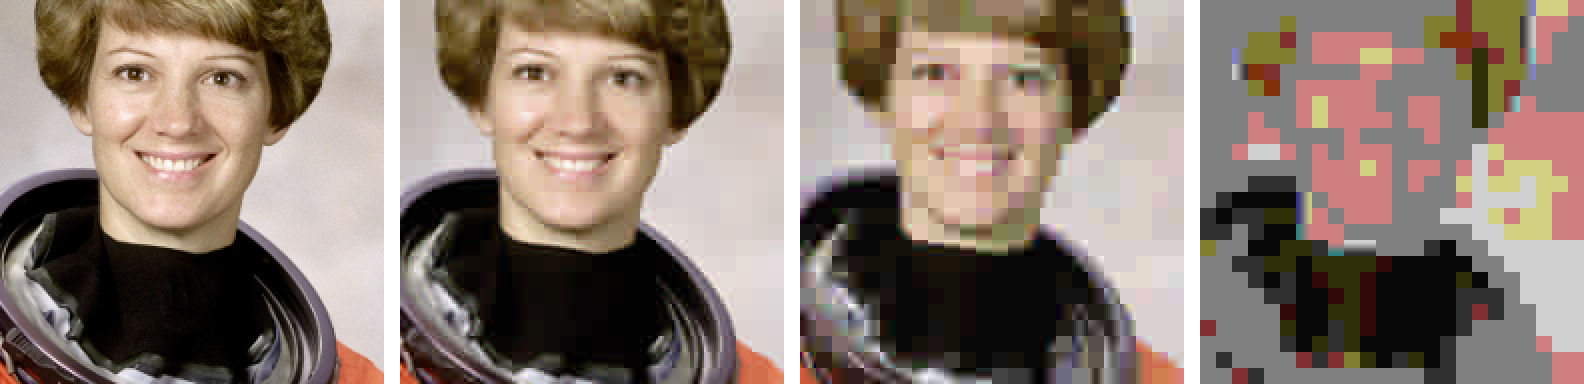
\includegraphics[width=0.8\textwidth]{figures/alpha.png}\\[0.1em]
  {\scriptsize
    \makebox[0.202\textwidth]{originale}%
    \makebox[0.202\textwidth]{$\alpha = 1$ : erreur 5,4\,\%}%
    \makebox[0.202\textwidth]{$\alpha = 5$ : erreur 11,3\,\%}%
    \makebox[0.194\textwidth]{$\alpha = 20$ : erreur 33\,\%}}
\end{frame}

\begin{frame}{Bilan : ce que le C++ nous a appris}
  \begin{columns}[T]
    \begin{column}{0.54\textwidth}
      \begin{itemize}
        \item \textbf{Le type porte l'information} : les hypothèses implicites du Python
          (multiples de 8, \code{int16}, fichier cohérent) deviennent des invariants
        \item \textbf{Chaque copie se voit} : \code{T}, \code{T\&} ou \code{const T\&},
          \code{std::array} ou \code{std::vector}, copie ou déplacement
        \item \textbf{La durée de vie structure le code} : RAII et règle de zéro, aucune
          gestion mémoire manuelle
      \end{itemize}
    \end{column}
    \begin{column}{0.42\textwidth}
      \textbf{Pour aller plus loin}
      \begin{itemize}
        \item zigzag et codage entropique (RLE, Huffman) : un vrai fichier JPEG
        \item espace YCbCr, sous-échantillonnage de la chrominance
        \item pointeurs intelligents pour conserver plusieurs masques
      \end{itemize}
    \end{column}
  \end{columns}
  \vspace{1.6em}
  \centering
  {\large\bfseries\color{accent} Merci, place aux questions}\\[0.4em]
  \small \url{https://github.com/BnRomain/jpeg-compression}
\end{frame}

\appendix
\renewcommand{\speaker}{Annexe}

\begin{frame}{Annexe : matrices de quantification}
  \centering
  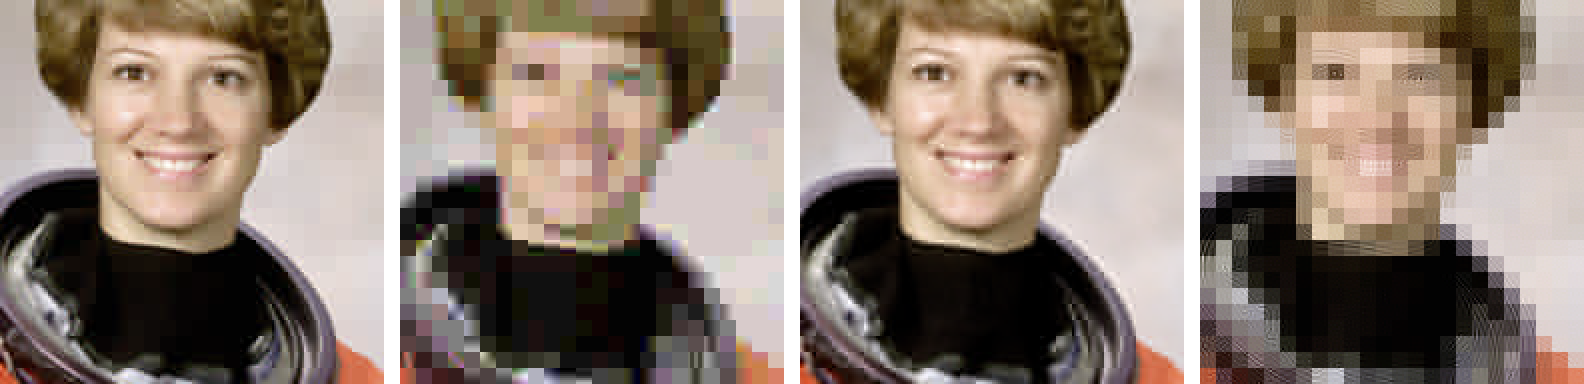
\includegraphics[width=0.9\textwidth]{figures/tables.png}\\[0.1em]
  {\scriptsize
    \makebox[0.2273\textwidth]{$Q$ standard}%
    \makebox[0.2273\textwidth]{$Q$ uniforme (100)}%
    \makebox[0.2273\textwidth]{basses fréquences}%
    \makebox[0.2181\textwidth]{hautes fréquences}}

  \vspace{0.5em}
  \small
  \begin{tabular}{@{}lrrr@{}}
    \toprule
    & Conservation & Erreur $L^2$ & Taille CSR \\
    \midrule
    $Q$ standard (psychovisuelle) & 5,79\,\% & 5,43\,\% & 273\,Ko \\
    $Q$ uniforme & 1,65\,\% & 13,85\,\% & 82\,Ko \\
    diviseurs faibles en basses fréquences & 8,76\,\% & 6,52\,\% & 409\,Ko \\
    diviseurs faibles en hautes fréquences & 25,45\,\% & 17,49\,\% & 1\,179\,Ko \\
    \bottomrule
  \end{tabular}
\end{frame}

\begin{frame}{Annexe : bruit poivre et sel}
  \centering
  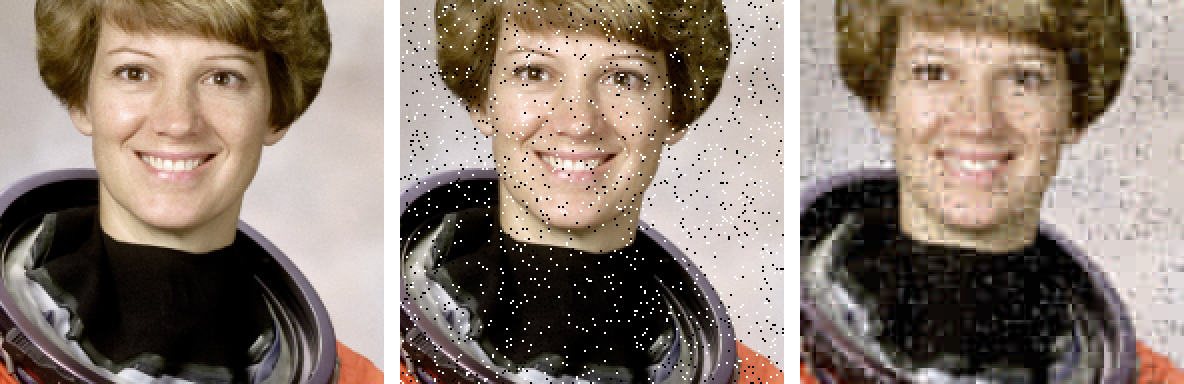
\includegraphics[width=0.8\textwidth]{figures/noise.png}\\[0.1em]
  {\scriptsize
    \makebox[0.2703\textwidth]{image pure}%
    \makebox[0.2703\textwidth]{bruitée à 5\,\%}%
    \makebox[0.2594\textwidth]{reconstruite, masque triangulaire $F = 4$}}

  \vspace{0.8em}
  \begin{columns}[T]
    \begin{column}{0.44\textwidth}
      \small
      Erreur $L^2$ par rapport à l'image pure :
      \begin{itemize}
        \item image bruitée : 24,0\,\%
        \item reconstruite, triangle $F = 4$ : 11,3\,\%
        \item reconstruite, réglages Python : 12,8\,\%
      \end{itemize}
    \end{column}
    \begin{column}{0.44\textwidth}
      \small
      Le bruit est fait de variations très rapides, donc de hautes fréquences :
      la troncature agit comme un filtre passe-bas, au prix d'un flou des contours.
    \end{column}
  \end{columns}
\end{frame}

\begin{frame}[fragile]{Annexe : utilisation}
\begin{lstlisting}[language=bash]
make && make test
./jpeg_csr compress images/astronaut.png --out results/standard
./jpeg_csr decompress results/standard/astronaut.csr decoded.png
\end{lstlisting}
  \vspace{0.2em}
\begin{lstlisting}[language={}]
Image          : images/astronaut.png (512 x 512, cropped to 512 x 512)
Settings       : Q standard, alpha 1.00, threshold 2, mask square F = 6
Coefficients   : 45566 non-zero out of 786432 (retention rate 5.79 %)
Quality        : relative L2 error 5.43 %, PSNR 30.49 dB
Dense memory   : 6144.00 KiB (float64, like img.nbytes)
CSR memory     : 273.00 KiB (int16 values, int32 indices)
Memory gain    : dense / CSR = 22.51x
.csr file      : 273.52 KiB, source image 773.00 KiB
Time           : compression 28.23 ms, decompression 21.55 ms
\end{lstlisting}
  \small Options : \code{--table standard|uniform|low|high}, \code{--alpha}, \code{--threshold},
  \code{--mask square|triangle}, \code{--cutoff}, \code{--noise}, \code{--out}.
\end{frame}

\end{document}
